\documentclass{article}

\usepackage[utf8]{inputenc}
\usepackage[a4paper, left=2cm, right=2cm, top=3cm, bottom=3cm]{geometry}
\usepackage{graphicx}
\usepackage{listings}
\title{Advaned Programming fo HPC - Report For Labwork 8}
\author{NGUYEN TAT HUNG M20.ICT.003}

\begin{document}

\maketitle

\section*{Implementation}
\begin{lstlisting}

import numba as nb;

import numpy as np
import timeit
import skimage.io as skio
from numba import cuda
import math

def dual_tuple_division(x, y):
    return_tuple = []
    for i, ii in zip(x, y):
        return_tuple.append(math.ceil(ii/i))
    return tuple(return_tuple)

@cuda.jit
def rgb_to_hsv(src, dst):
    i = cuda.threadIdx.x + cuda.blockIdx.x * cuda.blockDim.x
    j = cuda.threadIdx.y + cuda.blockIdx.y * cuda.blockDim.y
    r, g, b = src[i, j, 0], src[i, j, 1], src[i, j, 2]
    max_c = max(r, g, b)
    min_c = min(r, g, b)
    d = max_c - min_c

    # h
    if d == np.float64(0):
        dst[i, j, 0] = np.float64(0)
    if max_c == r:
        dst[i, j, 0] = 60 * ((g - b)/d % 6)
    if max_c == g:
        dst[i, j, 0] = 60 * ((b - r)/d + 2)
    if max_c == b:
        dst[i, j, 0] = 60 * ((r - g)/d + 4)

    # s
    if max_c == np.float64(0):
        dst[i, j, 1] = np.float64(0)
    if max_c != np.float64(0):
        dst[i, j, 1] = d/max_c

    # v
    dst[i, j, 2] = max_c


@cuda.jit
def hsv_to_rgb(src, dst):
    i = cuda.threadIdx.x + cuda.blockIdx.x * cuda.blockDim.x
    j = cuda.threadIdx.y + cuda.blockIdx.y * cuda.blockDim.y

    # preparation
    d = src[i, j, 0] / 60
    hi = np.uint8(d % 6)
    f = d - hi
    l = src[i, j, 2] * (1 - src[i, j, 1])
    m = src[i, j, 2] * (1 - f * src[i, j, 1])
    n = src[i, j, 2] * (1 - (1 - f) * src[i, j, 1])

    # conversion
    if np.float64(0) < src[i, j, 0] < np.float64(60):
        dst[i, j, 0], dst[i, j, 1], dst[i, j, 2] = src[i, j, 2], n, l
    if np.float64(60) <= src[i, j, 0] < np.float64(120):
        dst[i, j, 0], dst[i, j, 1], dst[i, j, 2] = m, src[i, j, 2], l
    if np.float64(120) <= src[i, j, 0] < np.float64(180):
        dst[i, j, 0], dst[i, j, 1], dst[i, j, 2] = l, src[i, j, 2], n
    if np.float64(180) <= src[i, j, 0] < np.float64(240):
        dst[i, j, 0], dst[i, j, 1], dst[i, j, 2] = l, m, src[i, j, 2]
    if np.float64(240) <= src[i, j, 0] < np.float64(300):
        dst[i, j, 0], dst[i, j, 1], dst[i, j, 2] = n, l, src[i, j, 2]
    if np.float64(300) <= src[i, j, 0] < np.float64(360):
        dst[i, j, 0], dst[i, j, 1], dst[i, j, 2] = src[i, j, 2], l, m

block_size_list = [(2,2),
                   (4, 4),
                   (8, 8),
                   (16, 16),
                   (32, 32)]

avgtime_list = []
for block_size in block_size_list:
    dtime_list = []
    for i in range(11):
        # Load and ignore alpha channel
        img = skio.imread('/content/drive/MyDrive/Colab Notebooks/tiger_driver.jpg')[:, :, :3]
        img = np.float64(img)
        img /= 255
        img = np.ascontiguousarray(img)
        h, w, c = img.shape
        out = np.array(img, copy=True)

        # Configure Cuda blocks
        grid_size = dual_tuple_division(block_size, (h, w))

        # Measure time
        stime = timeit.default_timer()
        A = cuda.to_device(img)
        B = cuda.to_device(out)
        rgb_to_hsv[grid_size, block_size](A, B)
        out = B.copy_to_host()
        skio.imsave('/content/drive/MyDrive/Colab Notebooks/rgb_to_hsv.png', np.uint8(out * 255))
        hsv_to_rgb[grid_size, block_size](B, A)
        B = A
        # Measure time
        dtime = timeit.default_timer() - stime
        dtime_list.append(dtime)

        out = B.copy_to_host()
        skio.imsave('/content/drive/MyDrive/Colab Notebooks/hsv_to_rgb.png', np.uint8(out * 255))

    avgtime = sum(dtime_list[1:])/len(dtime_list[1:])
    avgtime_list.append(avgtime)
    print(f'{avgtime} @ {block_size}')
    break




\end{lstlisting}
\section*{Result}
\begin{figure}[h]
\begin{center}
   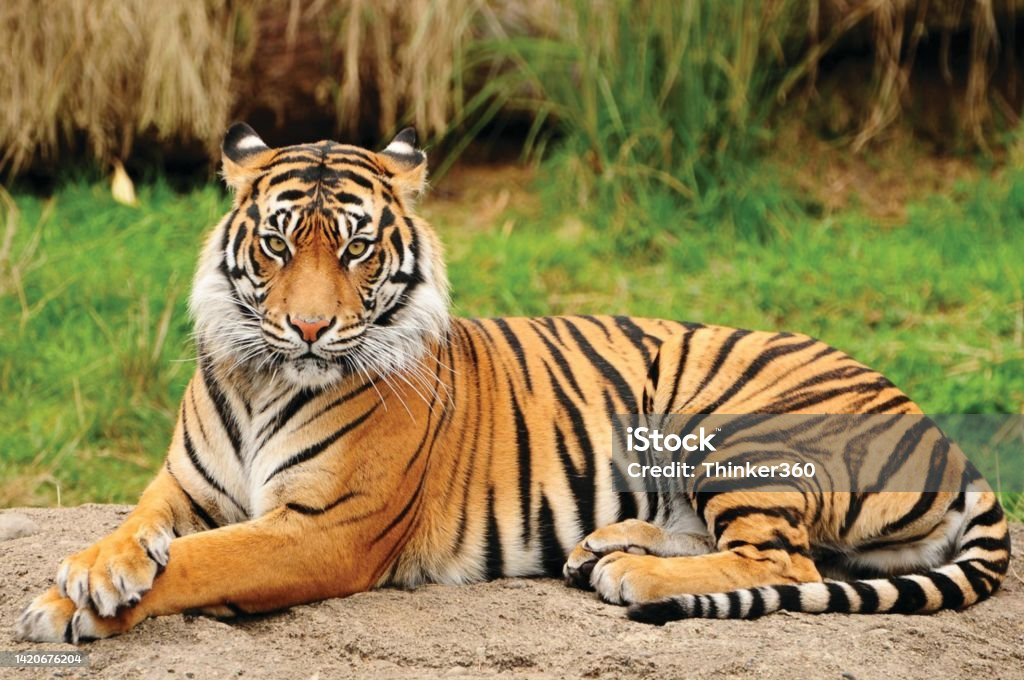
\includegraphics[scale=2]{tiger.jpg}
\end{center}
\caption{Original input image}
\end{figure}

\begin{figure}[h]
\begin{center}
   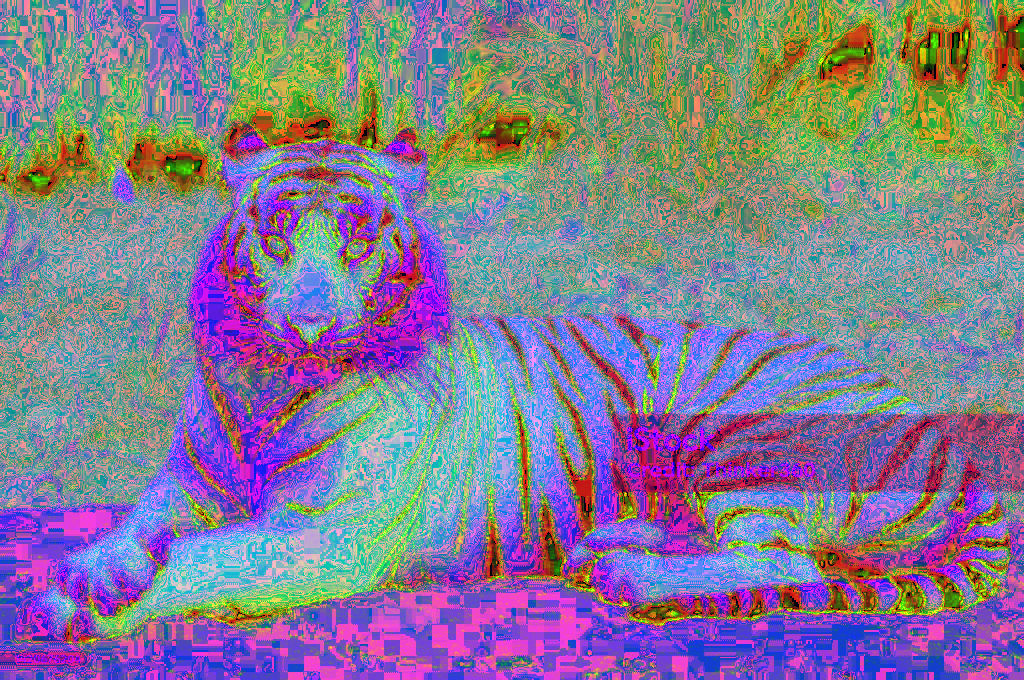
\includegraphics[scale=0.5]{rgb_to_hsv.png}
\end{center}
\caption{RGB to HSV image}
\end{figure}

\begin{figure}[h]
\begin{center}
   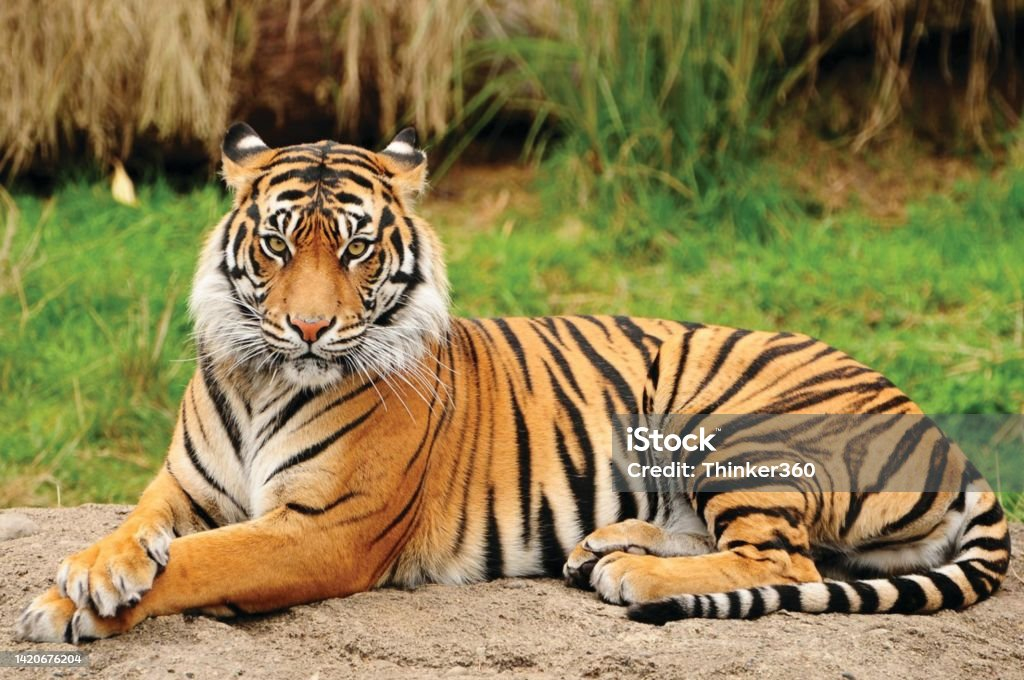
\includegraphics[scale=0.5]{hsv_to_rgb.png}
\end{center}
\caption{HSV to RGB image}
\end{figure}


\end{document}
